% Implicit encoding (DeepSDF + DGCI SDF loss) -- subsection of "Encoding",
% pulled in by sections/05-encoding.tex.
% Red \TODO{...} marks replace the [square-bracket] placeholders of the original draft.
%
% ==============================================================================
% REVISION NOTES
% ------------------------------------------------------------------------------
% Rewritten to match the code in Airway_Tree/DeepSDF: the model is the original
% DeepSDF auto-decoder (Park et al. 2019), trained with the SDF loss of DGCI
% (Zhang et al. 2024, Eqs. 3-4) instead of DeepSDF's clamped L1. Removed: shared
% code beta, hypernetworks, encoder-decoder, correspondence loss, intra/inter
% regularization. All values below were read from examples/airways_new/specs.json,
% train_deep_sdf.py, deep_sdf/dgci_loss.py, networks/deep_sdf_decoder.py,
% reconstruct.py and Dgci/normalized_SDF_points/run_batch.sh.
%
% Notation: the instance code is now z_i (DeepSDF's symbol) instead of alpha_i.
% If the clustering section refers to alpha_i, rename it there too.
% Old \label names (sec:dgci*, fig:dgci*, tab:dgci*) are kept as aliases
% so existing \secref / \ref calls elsewhere keep working. Equation labels are renamed
% eq:dgci_* -> eq:implicit_* (amsmath allows only one \label per equation).
% ==============================================================================

\subsection[Implicit encoding]{Implicit Neural Representation of Airway Trees}
\label{sec:implicit}                     % \secref{sec:implicit}
\label{sec:dgci}                         % old name, kept so existing references still work

The voxel-based models of \secref{sec:vae} and \secref{sec:ae} did not produce
satisfactory reconstructions. We therefore trained an implicit model: the DeepSDF
auto-decoder of \citet{park2019}, optimized with the signed distance loss proposed for
airway trees by \citet{zhang2024} instead of the original DeepSDF loss. This model gave the
best reconstructions of all the architectures we tested, and its learned latent codes are
the representation used for the clustering in \secref{sec:clustering}.

% ------------------------------------------------------------------------------
\subsubsection{Motivation}               % why an implicit representation
\label{sec:implicit_motivation}          % \secref{sec:implicit_motivation}
\label{sec:dgci_motivation}              % old name

Airway annotations are made slice by slice in CT image stacks, so the reconstructed shape is
inevitably limited by the resolution of the discrete voxels, and the image contrast degrades
as the bronchi become thinner. As a result, voxel-based airway trees tend to be coarse and
affected by spike-like noise, and CNN-based methods, which also work in the discrete voxel
space, suffer from the same problems as well as from breakages in the tree \cite{zhang2024}.

Implicit neural representations (INRs) address this by using coordinate-based neural
networks to parameterize a shape in continuous physical space instead of on a voxel grid.
They are therefore not bounded by the CT grid resolution, and they yield smoother shapes
with fewer spike-like artifacts \cite{park2019,zhang2024}. DeepSDF \cite{park2019} learns a
single network that represents a whole class of shapes, each shape being identified by a
low-dimensional latent code. These codes form a compact, continuous embedding of the
training shapes, which is what we need for clustering.

However, \citet{zhang2024} observed that the loss used by DeepSDF, an L1 penalty on the
predicted SDF values, is not sufficient to model fine airway structures with high fidelity.
They proposed additional geometric constraints, derived from implicit geometric
regularization \cite{gropp2020}, as part of their Deep Geometric Correspondence Implicit
(DGCI) model. We kept the DeepSDF architecture and adopted only this loss
(\secref{sec:implicit_loss}).
% [NOTE] If you also trained the full DGCI model (jobs/job_train_DGCI.sh) and it did worse,
% say so here in one sentence -- it justifies the choice of plain DeepSDF.

% ------------------------------------------------------------------------------
\subsubsection{Model}                    % auto-decoder + network
\label{sec:implicit_architecture}        % \secref{sec:implicit_architecture}
\label{sec:dgci_architecture}            % old name

\paragraph{Neural signed distance field.}  % the implicit function F
Each airway tree is represented by its signed distance function (SDF), which gives, for any
point in space, the distance to the closest point of the airway surface, with a negative
sign inside the lumen and a positive sign outside \cite{park2019}. A single neural network
$f_\theta$ represents the SDFs of all trees. It takes a coordinate
$\mathbf{p} \in \mathbb{R}^3$ together with a latent code $\mathbf{z}_i \in \mathbb{R}^K$
specific to the $i$-th airway tree, and predicts the signed distance of $\mathbf{p}$ to the
surface of that tree:
\begin{equation}
  \mathcal{F}(\mathbf{p}; \mathbf{z}_i) = f_\theta(\mathbf{z}_i, \mathbf{p})
  \approx \mathrm{SDF}_i(\mathbf{p}),
  \qquad f_\theta : \mathbb{R}^{K+3} \to \mathbb{R}.
  \label{eq:implicit_sdf}                % the neural SDF mapping
\end{equation}
The airway surface of tree $i$ is the zero level set of $\mathcal{F}(\cdot\,; \mathbf{z}_i)$,
and can be extracted as a mesh with Marching Cubes \cite{lorensen1987}.

\paragraph{Auto-decoder.}                % no encoder, codes are free parameters
DeepSDF has no encoder (Figure~\ref{fig:implicit_arch}). Instead, each training tree is
assigned a latent code $\mathbf{z}_i$ that is a free parameter, randomly initialized and
optimized jointly with the network weights $\theta$ by backpropagation
\cite{park2019}. After training, the decoder weights are fixed, and the code of a new tree
is obtained by optimizing $\mathbf{z}$ alone so that $\mathcal{F}(\cdot\,; \mathbf{z})$ fits
the samples of that tree (\secref{sec:implicit_inference}).

\paragraph{Network.}                     % layer sizes, skip connection
Following \citet{park2019}, $f_\theta$ is a multilayer perceptron with eight hidden
fully connected layers of 512 units, each with weight normalization \cite{salimans2016} and
no dropout. The input is the concatenation $[\mathbf{z}_i, \mathbf{p}]$, and the same vector
is concatenated again to the output of the fourth layer (skip connection). We use latent
codes of dimension $K = 256$.

\paragraph{Changes required by the geometric loss.}  % IGR-style modifications
The loss of \secref{sec:implicit_loss} constrains the spatial gradient
$\nabla_{\mathbf{p}}\mathcal{F}$, so training backpropagates through this gradient. We
therefore made three changes to the original DeepSDF network, following implicit geometric
regularization \cite{gropp2020}:
\begin{itemize}                          % the three architectural changes
  \item the ReLU activations are replaced by Softplus with $\beta = 100$, a smooth
        approximation of ReLU whose gradient is continuous, so that the gradient terms of
        the loss can themselves be differentiated;
  \item the final $\tanh$ is removed, because it bounds $|\mathcal{F}| < 1$ and flattens the
        output far from the surface, which conflicts with the unit-gradient (Eikonal)
        constraint;
  \item the weights are initialized with the geometric initialization of
        \citet{gropp2020}, so that before training the network approximates the SDF of a
        sphere of radius 0.5. The weights reading the latent code start at zero, so every
        tree starts from the same sphere.
\end{itemize}

\begin{figure}[htbp]                     % placeholder for the architecture diagram
  \centering                             % center the figure
  % 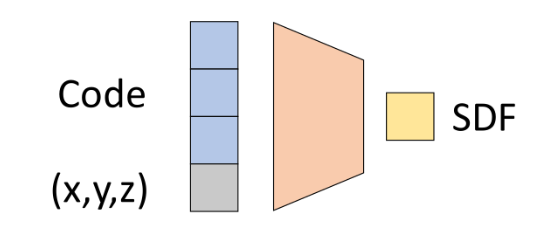
\includegraphics[width=\textwidth]{figures/deepsdf_architecture.png}  % uncomment with your file
  \fbox{\parbox[c][4cm][c]{0.9\textwidth}{\centering [DeepSDF auto-decoder figure]}}  % remove once image added
  \caption{The DeepSDF auto-decoder, adapted from \citet{park2019}. The latent code
           $\mathbf{z}_i \in \mathbb{R}^{256}$ of tree $i$ is concatenated with a query point
           $\mathbf{p}$ and passed through eight fully connected layers of width 512, with the
           input concatenated again after the fourth layer, to predict the signed distance
           $\mathcal{F}(\mathbf{p}; \mathbf{z}_i)$. The codes have no encoder: they are
           optimized together with the network weights.}
  \label{fig:implicit_arch}              % referenced as Figure~\ref{fig:implicit_arch}
  \label{fig:dgci_arch}                  % old name
\end{figure}

% ------------------------------------------------------------------------------
\subsubsection{Loss function}            % DGCI SDF loss + DeepSDF code regularization
\label{sec:implicit_loss}                % \secref{sec:implicit_loss}
\label{sec:dgci_loss}                    % old name



\paragraph{Sample sets.}                 % the three kinds of points per tree
For each tree $i$ of a mini-batch $\mathcal{B}$, three sets of points are drawn in every
iteration (\secref{sec:implicit_training}): surface points $S_i$, with their ground-truth
outward normals $\mathbf{n}'$; free-space points $V_i$ near and away from the surface, with
their ground-truth signed distances $s'$; and points $U_i$ drawn uniformly in the normalized
volume $[-1,1]^3$, which have no ground truth. On the surface, $s' = 0$. We write
$\Omega_i = S_i \cup V_i \cup U_i$ for all points of tree $i$, and, for a family of sets
$A_i$, $|A| = \sum_{i \in \mathcal{B}} |A_i|$ for its total number of points in the
mini-batch.

\paragraph{SDF loss.}                    % Eqs. 3-4 of Zhang et al. without beta
We use the SDF loss of \citet{zhang2024}, written here without their shared code, so that
$\mathcal{F}$ depends only on $\mathbf{z}_i$. It has two parts,
$\mathcal{L}_{\mathrm{sdf}} = \mathcal{L}_{\mathrm{sdf\text{-}val}} +
\mathcal{L}_{\mathrm{sdf\text{-}geo}}$, which supervise the values and the geometry of the
predicted SDF respectively:
\begin{equation}
  \mathcal{L}_{\mathrm{sdf\text{-}val}} =
  \frac{\omega_s}{|S \cup V|} \sum_{i \in \mathcal{B}} \sum_{\mathbf{p} \in S_i \cup V_i}
      \big|\mathcal{F}(\mathbf{p}; \mathbf{z}_i) - s'\big|
  + \frac{\omega_\varphi}{|U|} \sum_{i \in \mathcal{B}} \sum_{\mathbf{p} \in U_i}
      \varphi\big(\mathcal{F}(\mathbf{p}; \mathbf{z}_i)\big),
  \label{eq:implicit_val}                % SDF value term
\end{equation}
\begin{equation}
  \begin{split}
    \mathcal{L}_{\mathrm{sdf\text{-}geo}} =
    &\frac{\omega_n}{|S|} \sum_{i \in \mathcal{B}} \sum_{\mathbf{p} \in S_i}
        \big(1 - S_{\cos}(\nabla\mathcal{F}(\mathbf{p}; \mathbf{z}_i), \mathbf{n}')\big) \\
    &+ \frac{\omega_{\mathrm{Eik}}}{|\Omega|} \sum_{i \in \mathcal{B}} \sum_{\mathbf{p} \in \Omega_i}
        \big|\,\|\nabla\mathcal{F}(\mathbf{p}; \mathbf{z}_i)\|_2 - 1\big|,
  \end{split}
  \label{eq:implicit_geo}                % normal consistency + Eikonal term (split to fit)
\end{equation}
where $S_{\cos}$ is the cosine similarity and the gradient is taken with respect to
$\mathbf{p}$. Unlike \citet{zhang2024}, who sum over the points, we divide each term by the
number of points of its set in the mini-batch, so every term is a mean and the weights do
not depend on the number of samples.


% \paragraph{Sample sets.}                 % the three kinds of points per tree
% For each tree $i$, three sets of points are drawn in every iteration
% (\secref{sec:implicit_training}): surface points $S_i$, with their ground-truth outward
% normals $\mathbf{n}'$; free-space points $V_i$ near and away from the surface, with their
% ground-truth signed distances $s'$; and points $U_i$ drawn uniformly in the normalized
% volume $[-1,1]^3$, which have no ground truth. On the surface, $s' = 0$.

% \paragraph{SDF loss.}                    % Eqs. 3-4 of Zhang et al. without beta
% We use the SDF loss of \citet{zhang2024}, written here without their shared code, so that
% $\mathcal{F}$ depends only on $\mathbf{z}_i$. It has two parts,
% $\mathcal{L}_{\mathrm{sdf}} = \mathcal{L}_{\mathrm{sdf\text{-}val}} +
% \mathcal{L}_{\mathrm{sdf\text{-}geo}}$, which supervise the values and the geometry of the
% predicted SDF respectively:
% \begin{equation}
%   \mathcal{L}_{\mathrm{sdf\text{-}val}} = \sum_i \Big(
%   \omega_s \sum_{\mathbf{p} \in S_i \cup V_i}
%       \big|\mathcal{F}(\mathbf{p}; \mathbf{z}_i) - s'\big|
%   + \omega_\varphi \sum_{\mathbf{p} \in U_i}
%       \varphi\big(\mathcal{F}(\mathbf{p}; \mathbf{z}_i)\big)
%   \Big),
%   \label{eq:implicit_val}                % SDF value term
% \end{equation}
% \begin{equation}
%   \begin{split}
%     \mathcal{L}_{\mathrm{sdf\text{-}geo}} = \sum_i \Big(
%     &\omega_n \sum_{\mathbf{p} \in S_i}
%         \big(1 - S_{\cos}(\nabla\mathcal{F}(\mathbf{p}; \mathbf{z}_i), \mathbf{n}')\big) \\
%     &+ \omega_{\mathrm{Eik}} \sum_{\mathbf{p} \in S_i \cup V_i \cup U_i}
%         \big|\,\|\nabla\mathcal{F}(\mathbf{p}; \mathbf{z}_i)\|_2 - 1\big|
%     \Big),
%   \end{split}
%   \label{eq:implicit_geo}                % normal consistency + Eikonal term (split to fit)
% \end{equation}




% where $S_{\cos}$ is the cosine similarity and the gradient is taken with respect to
% $\mathbf{p}$. In practice, each sum is normalized by the number of points of its set in the
% mini-batch, so every term is a mean and the weights do not depend on the number of samples.

The first term of Equation~\eqref{eq:implicit_val} regresses the SDF values directly. Unlike
DeepSDF, which clamps both prediction and target to $[-0.1, 0.1]$ \cite{park2019}, it is
applied without clamping. The second term, with $\varphi(s) = \exp(-\delta |s|)$ and
$\delta = 100$, penalizes points away from the surface whose predicted SDF is close to zero,
and therefore suppresses spurious surfaces in empty space \cite{zhang2024}. \citet{zhang2024}
write this term over all off-surface points; we apply it, as in their released code, only to
the uniform points $U_i$, because many free-space points $V_i$ lie very close to the surface,
where a small SDF is correct and should not be penalized. Equation~\eqref{eq:implicit_geo}
aligns the SDF gradient with the surface normals and constrains its norm to one everywhere,
as required for a true distance function (Eikonal equation) \cite{gropp2020,zhang2024}.

\paragraph{Latent code regularization.}  % DeepSDF's prior on the codes
\citet{zhang2024} regularize their instance and shared codes and add a correspondence loss
for their encoder--decoder. Since our model has neither a shared code nor an
encoder--decoder, we keep instead the code regularization of the DeepSDF implementation,
which corresponds to a zero-mean Gaussian prior on the codes \cite{park2019}:
\begin{equation}
  \mathcal{L}_{\mathrm{reg}} = \lambda \, \min\!\Big(1, \frac{t}{100}\Big)
      \frac{1}{B} \sum_{i \in \mathcal{B}} \|\mathbf{z}_i\|_2,
  \label{eq:implicit_reg}                % code regularization with warm-up
\end{equation}
where $\mathcal{B}$ is the mini-batch of $B$ trees, $t$ the epoch, and $\lambda = 0.3$. The
factor $\min(1, t/100)$ increases the regularization linearly over the first 100 epochs. In
addition, the norm of every code is capped at 1.

\paragraph{Total objective.}             % what is minimized
The decoder weights $\theta$ and all training codes $\{\mathbf{z}_i\}$ are optimized jointly
by minimizing
\begin{equation}
  \mathcal{L}_{\mathrm{total}} = \mathcal{L}_{\mathrm{sdf\text{-}val}}
  + \mathcal{L}_{\mathrm{sdf\text{-}geo}} + \mathcal{L}_{\mathrm{reg}}.
  \label{eq:implicit_total}              % full training loss
\end{equation}
Following \citet{zhang2024}, we set $\omega_s = 3\times10^3$,
$\omega_\varphi = 5\times10^2$, $\omega_n = 10^2$ and $\omega_{\mathrm{Eik}} = 5\times10^1$.

% ------------------------------------------------------------------------------
\subsubsection{Data preparation and training}  % SDF sampling, optimizer, schedule
\label{sec:implicit_training}            % \secref{sec:implicit_training}
\label{sec:dgci_training}                % old name

\paragraph{Data.}                        % meshes, normalization, samples
Our dataset contains \TODO{N} airway trees from the AIIB23 \TODO{\cite{...}} and ATM22
\TODO{\cite{...}} datasets, split into \TODO{$N_{\mathrm{train}}$} training,
\TODO{$N_{\mathrm{val}}$} validation and \TODO{$N_{\mathrm{test}}$} test cases. Each airway
surface was extracted from its binary segmentation with Marching
Cubes \cite{lorensen1987}, and the SDF samples were prepared with the preprocessing of
DeepSDF \cite{park2019}. Each mesh is centered on its bounding box and scaled to fit in the
unit sphere with a margin of 3\%; the offset and scale are stored, so that predictions can
be mapped back to CT coordinates. Then, for each tree:
\begin{itemize}                          % the two sample files per tree
  \item 200,000 surface points with outward normals are obtained by rendering the mesh
        from virtual cameras placed around it and back-projecting the depth maps;
  \item 500,000 SDF samples are generated: 94\% near the surface, by perturbing surface
        points with Gaussian noise of variance $5\times10^{-4}$ and $5\times10^{-5}$, and
        6\% uniformly in $[-1,1]^3$. Their signed distance is the distance to the closest
        surface point, with the sign given by the orientation of the closest normals.
\end{itemize}
% [NOTE] Marching Cubes / mask-to-mesh step: confirm it is the one in jobs/job_nifti_to_mesh.sh.

\paragraph{Training.}                    % sampling per iteration, optimizer, schedule
In every iteration, we draw for each tree 4,096 surface points ($S_i$), 4,096 free-space
points ($V_i$), half of them inside and half outside the airway, and 2,048 uniform points
($U_i$). Balancing inside and outside samples is important for airways, since the lumen
occupies only a small fraction of the normalized volume and most samples are naturally
outside. The mini-batch contains $B = 64$ trees. The decoder weights and the latent codes
are optimized with Adam \cite{kingma2015}, with initial learning rates of $10^{-3}$ and
$2\times10^{-3}$ respectively, both halved every 4,000 epochs. The codes are initialized
from $\mathcal{N}(0, 1/K)$. The model was trained for \TODO{E} epochs on a single
\TODO{NVIDIA A100 / L40S} GPU. The training losses are shown in
Figure~\ref{fig:implicit_curves}.
% [NOTE] specs.json allows 20,001 epochs; report the epoch of the checkpoint you actually used.

After training, each training tree is represented by its latent code
$\mathbf{z}_i \in \mathbb{R}^{256}$. These codes are the features used for clustering in
\secref{sec:clustering}.

\paragraph{Latent codes of unseen trees.}  % test-time optimization
\label{sec:implicit_inference}           % \secref{sec:implicit_inference}
For validation and test trees, the decoder weights are frozen and only a new code
$\mathbf{z}$ is optimized \cite{park2019}. The code is initialized from
$\mathcal{N}(0, 0.01^2)$ and optimized for 800 iterations with Adam, with a learning rate of
$5\times10^{-3}$ divided by 10 after 400 iterations. The objective is the same SDF loss,
$\mathcal{L}_{\mathrm{sdf\text{-}val}} + \mathcal{L}_{\mathrm{sdf\text{-}geo}}$, on freshly
drawn samples of the tree, plus a prior term
$10^{-4}\,\omega_s \,\overline{\mathbf{z}^2}$, where $\overline{\mathbf{z}^2}$ is the mean of
the squared code entries.
% [NOTE] if the clustering uses only training codes, this paragraph is only needed for
% the validation/test reconstruction metrics below.

\begin{figure}[htbp]                     % placeholder for training curves
  \centering                             % center the figure
  % \includegraphics[width=\textwidth]{figures/deepsdf_training_curves.png}  % uncomment with your file
  \fbox{\parbox[c][4cm][c]{0.9\textwidth}{\centering [DeepSDF training loss curves]}}  % remove once image added
  \caption{Training losses of the DeepSDF model: total loss and the weighted terms of
           Equations~\eqref{eq:implicit_val}--\eqref{eq:implicit_reg} (SDF value, $\varphi$,
           normal, Eikonal and code regularization).}
  \label{fig:implicit_curves}            % referenced as Figure~\ref{fig:implicit_curves}
  \label{fig:dgci_curves}                % old name
\end{figure}
% [NOTE] the auto-decoder has no validation loss during training (validation codes are only
% fitted afterwards), so the old "training and validation losses" wording was removed.
% train_deep_sdf.py logs the per-term values each epoch; plot_log.py plots them.

% ------------------------------------------------------------------------------
\subsubsection{Evaluation metrics}       % continuous-space and voxel-space metrics
\label{sec:implicit_metrics}             % \secref{sec:implicit_metrics}
\label{sec:dgci_metrics}                 % old name

We follow the evaluation protocol of \citet{zhang2024}, which measures shape quality both in
continuous space, on the mesh extracted from the predicted SDF, and in discrete voxel space.
Meshes are extracted with Marching Cubes on a $\TODO{256}^3$ grid in the normalized volume.

\paragraph{Continuous space.}            % non-manifold counts on the mesh
Smoothness and connectivity of the reconstructed mesh are measured by counting non-manifold
(NM) elements. NM-V counts the vertices connected to three or more non-coplanar faces, NM-E
counts the edges shared by three or more faces, and NM-F counts the faces arranged in a way
that prevents a closed, continuous body from being formed. Fewer non-manifold elements
indicate better connectivity and smoothness \cite{zhang2024}.

\paragraph{Discrete space.}              % topology metrics on the voxelized result
To compute voxel-based metrics, the predicted SDF is evaluated directly on the voxel grid of
the original CT image: the center of each voxel is mapped to the normalized volume with the
stored offset and scale, and the voxel is labeled as airway if the predicted SDF is negative
\TODO{(with $2\times$ supersampling near the surface and a 50\% occupancy threshold)}. On this
volume we compute the tree length detected rate (TD) and the branch detected rate (BD),
defined in Eq.~\eqref{eq:td_bd}, and the Dice coefficient, which measure the topological
completeness and correctness of the reconstruction \cite{zhang2024}.
% [NOTE] this describes track_reconstruction.voxelize (same procedure as DGCI's create_mask).
% If your final evaluation used mesh voxelization + hole filling instead, revert to that.

% ------------------------------------------------------------------------------
\subsubsection{Results}                  % quantitative and qualitative results
\label{sec:implicit_results}             % \secref{sec:implicit_results}
\label{sec:dgci_results}                 % old name

Table~\ref{tab:implicit_results} reports the metrics on the \TODO{validation and test} sets,
and Figure~\ref{fig:implicit_recon} shows examples of reconstructed airway trees. This model
produced the best reconstructions of all the models we trained. \TODO{Describe the main
observations, e.g.\ preservation of fine distal branches, connectivity of the tree,
smoothness of the surface.}

\begin{table}[htbp]                      % quantitative results
  \centering                             % center the table
  \small                                 % slightly smaller font so the table fits
  \caption{Reconstruction results of the DeepSDF model trained with the SDF loss of
           \citet{zhang2024}, reported as mean $\pm$ standard deviation.}
  \label{tab:implicit_results}           % referenced as Table~\ref{tab:implicit_results}
  \label{tab:dgci_results}               % old name
  \begin{tabular}{lcccccc}               % set name + 6 metrics
    \toprule
    & \multicolumn{3}{c}{Continuous space} & \multicolumn{3}{c}{Discrete space} \\
    \cmidrule(lr){2-4} \cmidrule(lr){5-7}  % group underlines (lr = trim ends)
    Set & NM-V $\downarrow$ & NM-E $\downarrow$ & NM-F $\downarrow$
        & TD (\%) $\uparrow$ & BD (\%) $\uparrow$ & Dice (\%) $\uparrow$ \\
    \midrule
    Validation & \TODO{?} & \TODO{?} & \TODO{?} & \TODO{?} & \TODO{?} & \TODO{?} \\
    Test       & \TODO{?} & \TODO{?} & \TODO{?} & \TODO{?} & \TODO{?} & \TODO{?} \\
    \bottomrule
  \end{tabular}
\end{table}

\begin{figure}[htbp]                     % placeholder for reconstructions
  \centering                             % center the figure
  % \includegraphics[width=\textwidth]{figures/deepsdf_reconstructions.png}  % uncomment with your file
  \fbox{\parbox[c][4cm][c]{0.9\textwidth}{\centering [Original vs.\ reconstructed airway trees]}}  % remove once image added
  \caption{Ground-truth airway trees and their reconstructions by the DeepSDF model.}
  \label{fig:implicit_recon}             % referenced as Figure~\ref{fig:implicit_recon}
  \label{fig:dgci_recon}                 % old name
\end{figure}